

%------------------------------------------------------------%
\begin{frame}

\frametitle{Normal Distribution: Simulation Study}
\begin{itemize}
\item
Recall the experiment whereby a die was rolled 100 times, and the sum of the 100 values was recorded.
\item
This experiment was repeated a very large number of times (e.g. 100,000 times ) in a simulation study.
\item
A histogram was drawn to depict the distribution of outcomes of this experiment.


\end{itemize}
\end{frame}


\frame{
\frametitle{Normal Distribution: Simulation Study}

\begin{center}
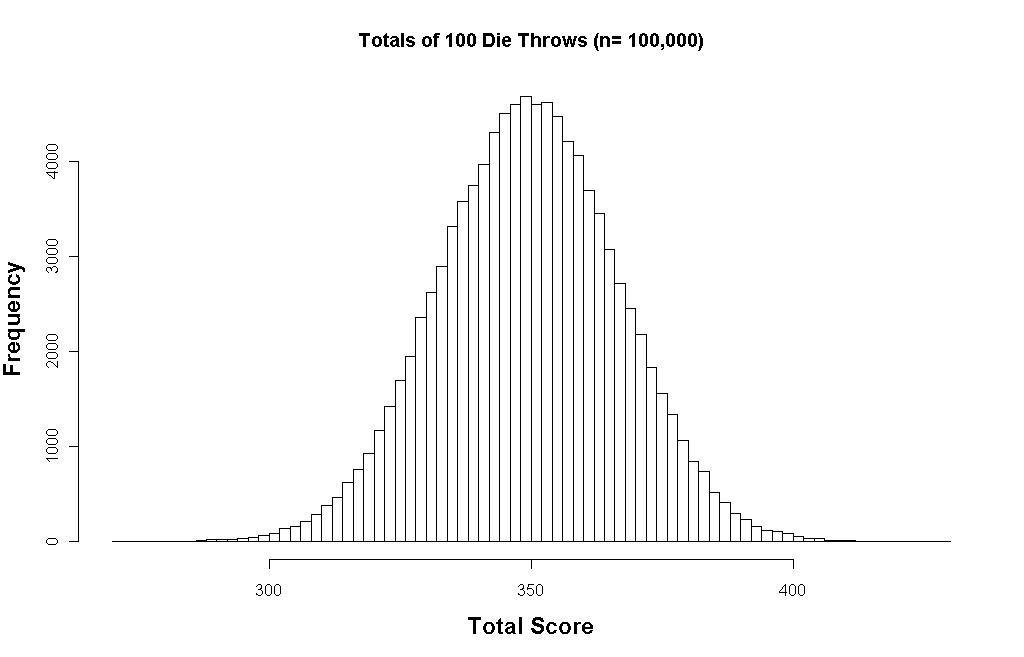
\includegraphics[scale=0.30]{images/3aDieHist3}
\end{center}

}

\frame{
\frametitle{Normal Distribution: Simulation Study}
Recall some observations made about the results of the simulation study, made in a previous lecture.
\begin{itemize}
% \item Approximately 76\% of the values are between 330 and 370.
\item Approximately 68.7\% of the values in the simulation study are between 332 and 367.
\item Approximately 95\% of the values are between 316 and 383.
\item $2.5\%$ of the values output are less than 316.
\item $2.5\%$ of the values study output are greater than 383.
\item 175 values are greater than or equal to 400, whereas 198 values are less than or equal to 300.
\item Results such as these are unusual, but they are not impossible.
\end{itemize}
}
%---------------------------------------------------------------%
\frame{
\frametitle{Normal Distribution: Simulation Study}
\begin{itemize}
\item Suppose we can \textbf{\emph{approximate}} the summation of the die-throws using the normal distribution.
\item The normal mean is necessarily $\mu = 350$.
\item The normal standard deviation is approximately 17. (68\% of values between $350 \pm 17$).
\item Using the normal distribution, lets estimate the proportion of values greater than 383.
\end{itemize}
}

%---------------------------------------------------------------%
\frame{
\frametitle{Normal Distribution: Simulation Study}

\begin{center}
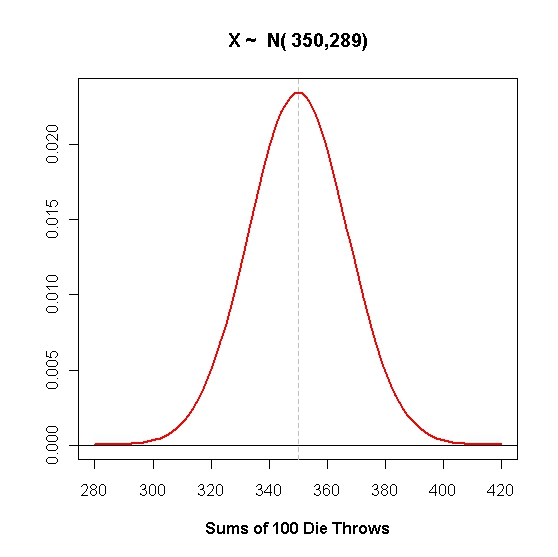
\includegraphics[scale=0.40]{images/5BNormalA}
\end{center}
}

%-------------------------------------------------------------%
\frame{
\frametitle{Normal Distribution: Simulation Study}
\begin{itemize}
\item X is the normal random variable that approximates the sum of values from 100 throws of a die.
\item Find $P(X \leq 383)$
\item First use the standardization formula to find the Z-score.
\[ z_o = {383 - 350 \over 17} = {33 \over 17} = 1.94 \]
\item Use the tables to compute $P(Z \geq 1.94)$ (\alert{Answer: 0.0262} )
\item Because $P(Z \geq 1.94)  = 0.0262$, we can say $P(X \geq 383)  = 0.0262$
\item This is close to the proportion of observed values, which was 2.5\%.
\item Remark : The standard deviation of 17 was an estimate. The actual standard deviation should 17.12.
\end{itemize}
}

\frame{
\frametitle{Normal Distribution: Simulation Study}

\begin{center}
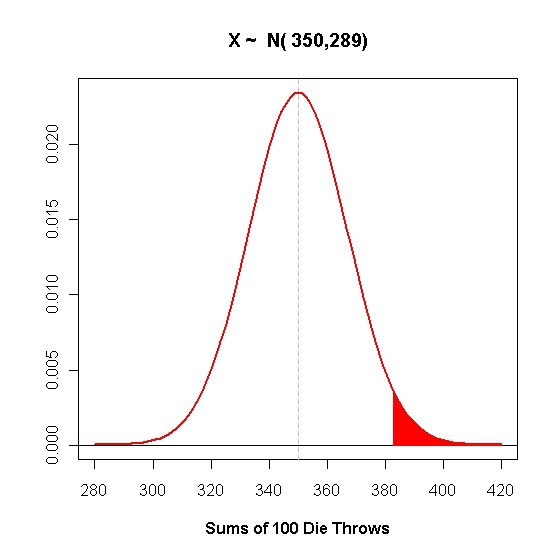
\includegraphics[scale=0.40]{images/5BNormalB}
\end{center}

}


